% Chapter 6

\chapter{RESULTS AND DISCUSSION} % Write in your own chapter title

\section{Results}
\subsection{Assessment}


\begin{figure}[H]
  \centering
  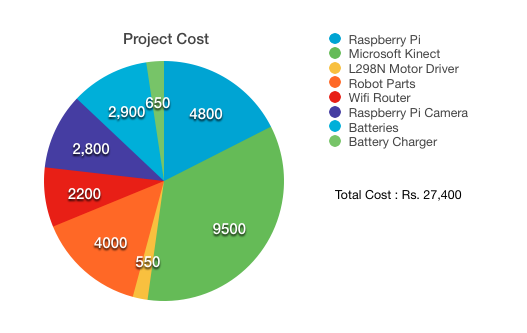
\includegraphics[width = 15cm, height = 9cm, scale=1]{graph4.png}
  \caption{Project Cost for each Part}
  \label{Cost wise Estimate}	
\end{figure}

\begin{table}[H]
    \begin{tabular}{ | l | l | l | p{1cm}|}
    \hline
    S.No & Signal & Result \\ \hline
    1 & Swipe left joystick up & Quadcopter flies upward \\ \hline
    2 & Swipe left joystick down &  Quadcopter's height decreases \\ \hline
    3 & Swipe right joystick up & Quadcopter pitches forward \\ \hline
    4 & Swipe right joystick down & Quadcopter pitches backward \\ \hline
 5 & Swipe right joystick left & Quadcopter pitches left \\ \hline
 6 & Swipe right joystick right & Quadcopter pitches right \\ \hline
 7 & Click the 'start' camera button & Pi Camera starts shooting \\ \hline
 8 & Click the 'stop' camera button & Pi Camera stops shooting \\ \hline
 9 & Click the '+/-' button on the x-axis & Quadcopter's x-trim values change \\ \hline
 10 & Click the '+/-' button on the y-axis & Quadcopter's y-trim values change \\ \hline
\end{tabular}
\caption{Test Cases and Results}
\label{APT}
\end{table}

\subsection{Evaluation}
There are several changes that have to be made when flying the quadcopter in varying environments. The PID values change according to the wind conditions and other disturbances. Although the SD Card is securely inserted into the RPi, due to a large amount of vibration caused in the course of the quadcopter's flight, it may loosen leading to connection loss between the RPi and the App. The quadcopter is controlled by the App from a distance of about 10-15 metres since communication occurs via WiFi. Images are taken by a RPi native camera. The quality of the images taken largely depend on the stability of the quadcopter which are subject to the vagaries of the environment.
The pictures taken are stitched and/or reconstructed. This process depends on the number of images taken and the quality of the images. 
\begin{figure}[H]
  \centering
  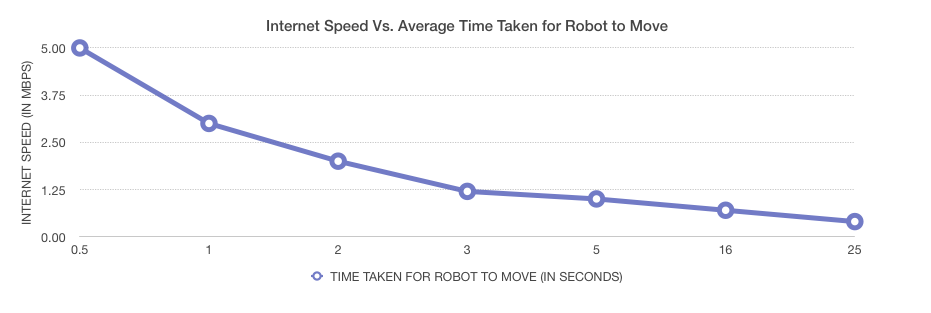
\includegraphics[width = 15cm, height = 7cm]{graph2.png}
  \caption{Time taken for Robot to Move based on Internet Speed}
  \label{Internet speed based performance}	
\end{figure}


\begin{figure}[H]
  \centering
  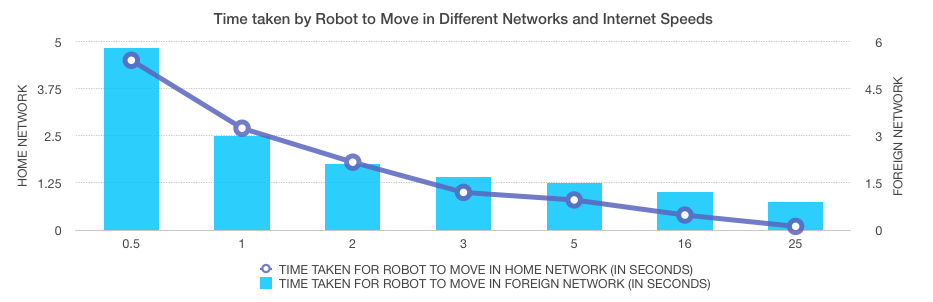
\includegraphics[width = 15cm, height = 6cm]{graph1.png}
  \caption{Time taken for Robot to Move in Different Networks based on Internet Speed}
  \label{Network based performance}	
\end{figure}

\begin{figure}[H]
  \centering
  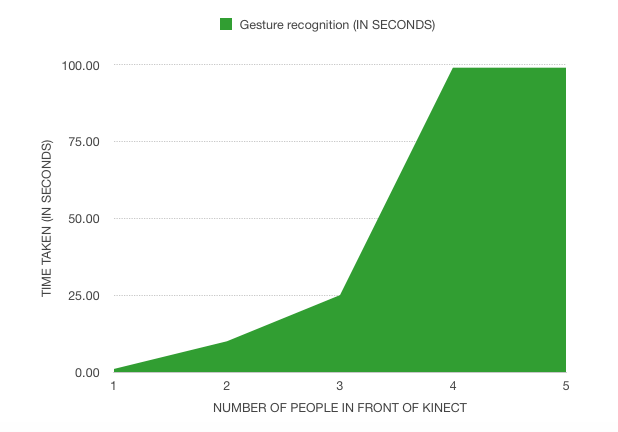
\includegraphics[width = 15cm, height = 11cm]{graph3.png}
  \caption{Time taken to Recognise Gesture based on Number of People in Front of Kinect}
  \label{Kinect performance}	
\end{figure}


\begin{figure}[H]
  \centering
  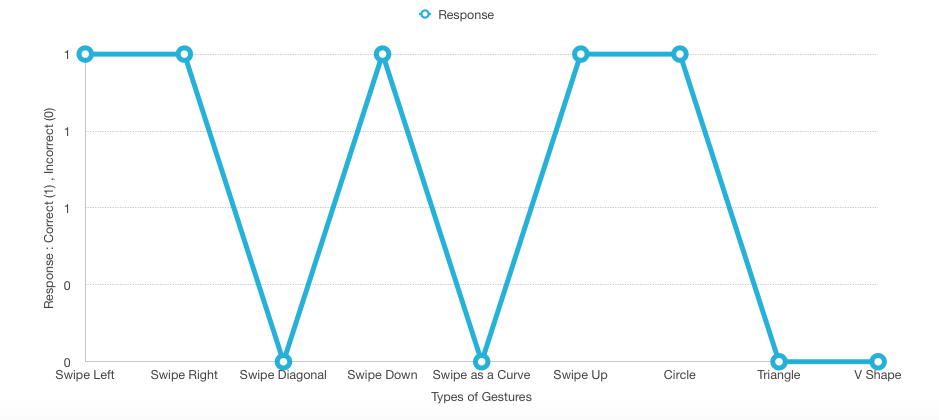
\includegraphics[width = 15cm, height = 7cm]{graph5.png}
  \caption{Response based on type of gesture}
  \label{Gesture-action pair}	
\end{figure}


